%% Credits of this ams template are with respective people. @Devansh1106 neither own this template nor the credits. 
\documentclass[reqno,10pt]{amsart}
\usepackage[a4paper, margin=1.25in]{geometry} % Change 1in to desired size
\usepackage[numbers]{natbib}
\setlength{\bibsep}{8pt}
\usepackage{dsfont}
\usepackage{graphicx}
\usepackage{tikz-cd}
\usepackage{subcaption}
% \captionsetup[subfigure]{labelformat=parens,labelfont=normalfont}
% \renewcommand{\thesubfigure}{\alph{subfigure}}
\usepackage{hyperref}
\usepackage{lineno}
\usepackage{amssymb}
\usepackage{amsmath}
\usepackage{amsthm}
\usepackage{mathtools}
\usepackage{mathrsfs}
\usepackage{esint}
\usepackage{fancyhdr}

\DeclareMathAlphabet{\EuScript}{U}{eus}{m}{n}

\setlength{\parskip}{0.5\baselineskip}%
\setlength{\parindent}{20pt}
\theoremstyle{plain}

\pagestyle{fancy}
\fancyhf{} % Clear default headers/footers
\setlength{\headheight}{10.0pt}
% Even pages: Paper title
\fancyhead[LE]{\footnotesize\textit{Universality of POSEIDON in settings of ANOs}}

% Odd pages: Author name
\fancyhead[RO]{\footnotesize\textit{Devansh Tripathi}}

\newtheorem*{thm*}{Theorem}
%% this allows for theorems which are not automatically numbered
\newcommand{\sinc}{\text{sinc}}
\renewcommand{\qedsymbol}{$\blacksquare$}
\newtheorem{thm}{Theorem}
\newtheorem{cor}{Corollary}
\newtheorem{lem}{Lemma}
\newtheorem*{lem*}{Lemma}
\newtheorem{prop}{Proposition}
\theoremstyle{definition}
\newtheorem{defn}{Definition}
\newtheorem{eg}{Example}
\newtheorem{rem}{Remark}
\newcommand{\bb}[1]{\mathbb{#1}}
\newcommand{\cal}[1]{\mathcal{#1}}
\newcommand{\eus}[1]{\EuScript{#1}}

\hypersetup{
    colorlinks=false,
    linkcolor=blue,    % Internal links (sections, equations)
    citecolor=red,     % Citation links
    urlcolor=magenta   % URLs (DOIs, websites)
}
%% The above lines are for formatting.  In general, you will not want to change these.

\title{Report on the paper ``{\Large P}OSEIDON: Efficient Foundation Models for PDEs''}
\author{Devansh Tripathi$^1$ \\ ETH Z\lowercase{\"urich}}
\thanks{$^1$Seminar für Angewandte Mathematik, HG E 62.2, Rämistrasse 101, 8092 Zürich, Switzerland \\ \href{mailto:devansh.tripathi@sam.math.ethz.ch}{\texttt{devansh.tripathi@sam.math.ethz.ch}}}

\begin{document}
\numberwithin{equation}{section}

\begin{abstract}
    In the paper \cite{MH2024}, the author introduces a foundation model {\large P}OSEIDON, for learning the solution operators of PDEs. It is based on a multiscale operator transformer, with time-conditioned layer norms that enable continuous-in-time evaluations. They propose a novel training strategy leveraging the semi-group property of time-dependent PDEs to allow for significant scaling-up of the training data. {\large P}OSEIDON is a pretrained model on a diverse, large scale dataset for the governing equations of fluid dynamics. The authors show that {\large P}OSEIDON exhibits excellent performance by outperforming baselines significantly, both in terms of sample efficiency and accuracy. They also show the generalization ability of the model to unseen physics.
\end{abstract}
\maketitle
\section{\bf Introduction}
\noindent Partial Differential Equations (PDEs) are referred to as the language of physics as they mathematically model a very wide variety of physical phenomena across a vast range of spatio-temporal scales. Numerical methods such as finite difference, finite element, spectral methods etc. are commonly used to approximate or simulate PDEs. However, their (prohibitive) computational cost, particularly for the so-called many-query problems, has prompted the design of various data-driven machine learning (ML) methods for simulating PDEs. Among them, operator learning algorithms have gained increasing traction in recent years.

\noindent These methods aim to learn the underlying PDE solution operator, which maps function spaces inputs (initial and boundary condition, coefficients, sources) to the PDE solution. They include algorithms which approximate a {\it discretization}, on a fixed grid, of the underlying solution operator. These can be based on convolutions \cite{YZ2018}, graph neural network \cite{TP2021,ASG2020} or transformers \cite{MP2022,ZH2023}. Other operator learning alogorithms are {\it neural operators} which can directly process function space input and outputs, possibly sampled on multiple grid resolutions. These include DeepONets \cite{LL2021}, Fourier Neural Operator \cite{ZL2021}, CNO \cite{BR2023}, among many others.

\paragraph{\bf How can the number of training samples for PDE learning be significantly reduced?} 
{\it Foundation models} are {\it generalist} models that are pretrained, at-scale, on laarge datasets drawn from a diverse set of data distributions. They leverage the intrinsic abilitiy of neural networks to learn {\it effective representations} from pretraining and are then successfully deployed on a variety of {\it downstream} tasks by {\it finetunning} them on a few task-specific samples. Example of such models include highly successful large language models \cite{HT2023}.

\noindent The challenge of designing such foundation models for PDEs is formidable given the sheet variety of PDEs and data distributions. Authors concur that the feasibility of of designing PDE foundation models rests on the fundamental and unanswered science question of {\it why pretraining a model on a very small set of PDEs and underlying data-distributions can allow it to learn effective representations and generalize to unseen and unrelated PDEs and data-distributions via finetuning?}

\noindent The Poseidon family of PDE foundation models are based on i) scalable Operator Transformer or scOT, a {\it multiscalae vision transformer} with (shifted) windowed or Swin attention \cite{ZLiu2021}, adapted for operator learning, ii) a novel all2all training strategy for efficient leveraging {\it trajectories} of solutions of time-dependent PDEs to scale up the volume of training data and iii) an open source large-scale pretraining dataset, containing a set of novel solution operators of the compressible Euler and incompressible Navier-Stokes equations of fluid dynamics.

\section{\bf Approach}
\paragraph{\bf Problem Formulation} We denote a generic time-dependent PDE as,
\begin{equation}\label{eq:pde}
    \begin{split}
        &\partial_t u(x,t) + \cal L(u, \nabla_x u_x, \nabla^2_x u, \dots) = 0, \quad \forall x \in D \subset \bb R^d, t \in (0,T), \\
        &\cal B(u) = 0, \quad \forall(x,t) \in \partial D \times (0,T), \quad u(0,x) = a(x), \quad x \in D
    \end{split}
\end{equation}
Here, with a function space $\EuScript{X} \subset L^p(D;\bb R^n)$ for some $1 \leq p < \infty, u \in C([0,T];\EuScript X)$ is the solution of ((\ref{eq:pde})), $a \in \EuScript X$ the initial datum and $\cal L, \cal B$ are the underlying differential and boundary operators, respectively. Note that (\ref{eq:pde}) accomodates both PDEs with high-order time derivatives as well as  PDEs with (time-independent) coefficients and sources by including the underlying functions within the solution vector and augmenting $\cal L$ accordingly.

\noindent Even {\it time-independent} PDEs can be recovered from (\ref{eq:pde}) by taking the {\it long-time limit}, i.e., $\lim_{t \to\infty} u = \overline{u}$, which will be the solution of the (generic) time-independent PDE,
\begin{equation}
    \cal L(\overline{u}(x), \nabla_x \overline{u}, \nabla^2_x\overline{u}, \dots) = 0, \quad \forall x \in D, \quad \cal B(\overline{u}) = 0, \quad \forall x \in \partial D.
\end{equation}
Solutions of the PDE (\ref{eq:pde}) are given in terms of the underlying {\it solution operator} $\EuScript S: [0,T] \times \eus X \mapsto \eus X$ such that $u(t) = \eus S(t,a)$ is the solution of \ref{eq:pde} at any time $t \in (0,T)$. Given a data distribution $\mu \in Prob(\eus X)$, the {\it underlying operator learning task (OLT)} is,

\begin{quote}
    {\bf OLT}: {\it Given any initial datum $a \sim \mu$, find an approximation $\eus S^* \approx \eus S$ to the solution operator $\eus S$ \ref{eq:pde}, in order to generate the entire solution trajectory \{$\eus S^*(t,a)\}$ for all $t\in [0,T]$.}
\end{quote}
It is essential to emphasize here that the learned opeator $\eus S^*$ has to generate the {\it entire solution trajectory for \ref{eq:pde}, given only the initial datum (and boundary conditions),} as this is what the underlying solution operator $\eus S$ (and numerical approximation to it) does.

\paragraph{\bf Model Architecture} The backbone for the {\large P}OSEIDON foundation model is provided by scOT or {\it scalable Operator Transformer,}. scOT is a {\it hierarchical multiscale vision transformer with lead-time conditioning} that processes lead time $t$ and function space valued initial data input $a$ to appropriate the solution operator $\eus S(t,a)$ of the PDE \ref{eq:pde}.

\noindent As in a vision transformer \cite{AD2021}, any underlying input is first {\it partitioned into patches and (linearly) embedded into a latent space}. At the level of function inputs $a \in C(D;\bb R^n)$, this amounts to the action of the patch {\it patch partitioning and embedding} operator $v = \hat{\bf E}(a)$, with $\hat{\bf E}$ defined in \ref{eq:embeddop}. This operator transforms the input function into a piecewise constant function, which is constant within patches (subdivisions of the domain $D$), by taking the weighted averages and then transforming these piecewise constant values into a $C$-dimensional latent space resulting in output $v \in C(D;\bb R^C)$.
\begin{figure}[!ht]
    \centering
    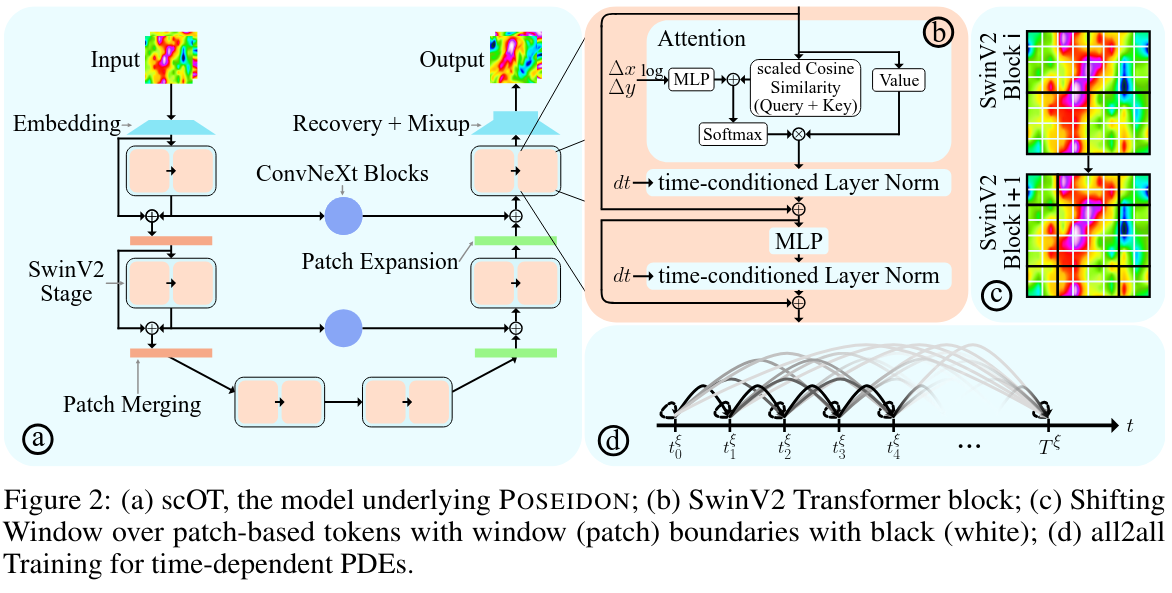
\includegraphics[width=\textwidth]{poseidon_arch.png}
    \caption{Taken from \cite{MH2024}}
    \label{fig:architecture}
\end{figure}

\noindent As shown in Figure \ref{fig:architecture}, this patch embedded output is then processed through a sequence of {\it SwinV2 transformer} blocks \cite{ZL2022,ZLiu2021}, each of which has a structure of $SW_l : C(D;\bb R^C) \mapsto C(D;\bb R^C)$,
\begin{equation}\label{eq:swinv2}
    \begin{aligned}        
        {\bf v_l} = SW_l({\bf v}_{l-1}) &= {\bf v'}_l + LN_{\alpha^l_2, \beta_2^l}(MLP({\bf v'}_l)), \\
        {\bf v'}_l &= {\bf v}_{l-1} + LN_{\alpha_1^l, \beta_1^l} (W-MSA({\bf v}_{l-1})).
    \end{aligned}
\end{equation}
for layer index $ l = 1, \dots ,L$. The main building block of a SwinV2 transformer block \ref{eq:swinv2} is the {\it windowed multi-head self attention} operator defined in \ref{eq:wmsa}. The attention operator acts only inside window and the windows are shifted across layers so that all points in the domain can be attended to.

\noindent The MLP is \ref{eq:swinv2}, is defined in \ref{eq:mlp}. Author follows \cite{EP2017} to propose a {\it time-conditioning} strategy by introducing a {\it lead-time conditioned} layer norm in \ref{eq:swinv2},
\begin{equation} \label{eq:LN}
    \begin{aligned}
        LN_{\alpha(t),\beta(t)}({\bf v})(x) &= \alpha(t) \odot \frac{{\bf v}(x) - \mu_{{\bf v}}(x)}{\sigma_{\bf v}(x)} + \beta(t), \\
        \mu_{{\bf v}}(x) &= \frac{1}{C}\sum_{j=1}^{C} {\bf v}_j(x), \quad \sigma_{{\bf v}}^2(x) = \frac{1}{C} \sum_{j=1}^{C} ({\bf v}_j(x) - \mu_{{\bf v}}(x))^2,
    \end{aligned}
\end{equation}
Here $\alpha(t) = \alpha t + \overline{\alpha}$ and $\beta(t) = \beta t + \overline{\beta}$, with learnable $\alpha, \overline{\alpha}, \beta, \overline{\beta}$ although more general (small) MLPs can also be considered. This choice of time embedding enables {\it continuous-in-time evaluations}.

Finally, as in Figure \ref{fig:architecture}, the SwinV2 transformer blocks \ref{eq:swinv2} are arranged in a hierarchical, multiscale manner, within a U-Net style {\it encoder-decoder} architecture, by employing patch merging (downscaling) and patch expansion (upscaling) operator. Moreover, layers at the same scale, but within the encoder and decoder stages of scOT, respectively, are connected through {\it ConvNeXt} convolutional layers \cite{ZLiu2022}.

\section{\bf Universal Approximation of POSEIDON}
\noindent This section deals with proving that the underlying architecture of POSEIDON is universal by showing that the building blocks of POSEIDON can proved to be equivalent to ANOs \cite{SL2024}, and then we utilize the universality of ANOs to show that POSEIDON is indeed a universal approximator.

\begin{lem}[{\bf ConvNeXt is an ANO}] \label{lem:convnext}
    ConvNeXt blocks are given by
    \begin{equation}
        \cal Q_i({\bf v},t) = (\text{GeLU}(LN(DwConv({\bf v}),t)W_{\cal Q,1}+b_{\cal Q,1})W_{\cal Q,2} + b_{\cal Q,2}) \odot W_{\cal Q,3} + {\bf v}.
    \end{equation}
    where $\text{DwConv}$ is a depthwise convolution with kernel size $7$. With the following choice: taking all weight matrices to be identity matrix, $W_{\cal Q, 3}$ as vector of $1's$ and all bias vector to zero vectors then we have a reduced form as
    \begin{equation}
        \cal Q_i({\bf v},t) = \text{GeLU}(LN(DwConv({\bf v}),t)) + {\bf v}.
    \end{equation}
    This is an ANO and by Theorem 2.1 in \cite{SL2024}, ConvNeXt is universal approximator.
\end{lem}
\begin{proof}
    The convolution given by DwConv can be represented as an integral and this will provide nonlocality to the network. Let $\cal K_l(v)$ be the convolution operator given by
    $$(\cal K_lv)(x) = \int_{D} K_l(x,y) v(y) dy.$$
    The particular choice $K_l(x,y) \equiv |D|^{-1} I_{7\times 7}$ with $I_{7\times 7}$ be the identity matrix, it recovers the form of average as in ANO \cite{SL2024}. 
    \paragraph{\bf Layer Norm}\label{par:LN} If we choose $\alpha(t)$ to be vector of $1$'s and $\beta(t)$ to be zero vector in LN (time conditioned layer norm as in \ref{eq:LN}) then LN only changes the first and second moments of the entries of the vector ${\bf v}(x)$ and the affine transformation becomes identity transform due the above choices. Overall output still captures the nonlocality needed for the ANO because of the integral and just changes the numerical values of the entries of the vector. Hence, it is still nonlocal and appyling LN does not affect the nonlocailty.
    $$ LN_{\alpha(t),\beta(t)}({\bf v})(x) = \alpha(t) \odot \frac{{\bf v}(x) - \mu_{{\bf v}}(x)}{\sigma_{\bf v}(x)} + \beta(t) = \frac{{\bf v}(x) - \mu_{{\bf v}}(x)}{\sigma_{\bf v}(x)} $$
    \paragraph{\bf Residual connection} \label{par:resano} Applying residual connection mathematically means shifting the output vector of GeLU. It is required to take care of the issue of vanishing gradients while training. In particular the bias vector in the hidden layer of the ANO will absorbs the shift provided by residual connection and it will not affect the ANO. Hidden layer of ANO with residual connection is given by
    $$ v_l(x) = \underbrace{\sigma\left(Wv_{l-1}(x) + b + \fint v_{l-1}(y)dy\right)}_{\text{Original ANO}} + \underbrace{v_{l-1}(x)}_{\text{Residual connection}} $$
    Hence $v_{l-1}(x) = v_{l-2}(x) + v'(x)$ where $v'(x) = \sigma\left(Wv_{l-2}(x) + b + \fint v_{l-2}(y)dy\right) $ be the output vector of original ANO without residual connection, then
    \begin{equation*}
        \begin{aligned}
            v_l(x) &= \sigma\left(Wv_{l-1}(x) + b + \fint (v_{l-1}(y) + v'(y))dy\right) + v_{l-1}(x) \\
            &= \sigma\left(Wv_{l-1}(x) + b + \fint v_{l-1}(y) dy + \fint v'(years) dy\right) + v_{l-1}(x) \\
            &= \sigma\left(Wv_{l-1}(x) + b' + \fint v_{l-1}(y) dy \right) + v_{l-1}(x)
        \end{aligned}
    \end{equation*}
    where $b' = b + \fint v'(y)dy$ be a new bias vector. Hence the core structure of ANO is still preserved even with the shifted input and the core structure is proved to be universal in \cite{SL2024} which makes this {\bf {\it ResANO} (ANO with a residual connection) a universal approximator}

    \noindent In particular, the ConvNeXt block is a type of {\it ResANO} as shown above that it has ANO type nonlocailty and a residual connection. Hence, it is an universal approximator.
\end{proof}
\paragraph{\bf Setup} \label{par:setup} Now we show that the windowed multi-head self attention is equivalent to averaging. Notice that we can choose the query, key and value matrices, $Q_l = XW^Q$, $K = XW^K$ and $V = XW^V$ respectively, where $X \in \bb R^{m \times C}$, $m$ is the total number of patches and $X$ is the input sequence vector. Here $W^*$ are the trainable matrices in $\bb R^{C\times C}$. For the proof of the lemma below, we set $m = 1$ and $W^V = X^\dag$ (pseudo inverse of $X$) then the above quantities will be simplified: $X \in \bb R^{1\times C}$, $Q_l, K_l$ and $V_l$ will be in $\bb R^{1\times C}$. With these choices, we have the following lemma.
\begin{lem}[{\bf W-MSA is equivalent to average}]\label{lem:wmsa}
    Windowed multi-head self attention as given by \ref{eq:wmsa} is equivalent to averaging with $Q_l, K_l$ and $V_l$ as given in the above paragraph and the following choices: take ${\bf W}^h_l = \alpha^{-1}\bb I$ where $\bb I$ is identity matrix and $\alpha = XX^\dag$, H = 1 (number of attention head, without loss of generality), $D^l_{q_x} = D~~ \forall l$ and ${\bf B}_l(x,y)$ to be a zero vector. Then we have a simplified version of W-MSA as
    $$W-MSA(v)(x) = \alpha^{-1}\int_{D} \frac{e^{cos({\bf Q}_l {\bf v}(x),{\bf K}_l {\bf v}(y))}}{\int_{D} e^{cos({\bf Q}_l {\bf v}(z),{\bf K}_l {\bf v}(y))}dz} {\bf V}_l {\bf v}(y) dy.$$
    This is equivalent to the nonlocailty of ANO (averaging over the domain).
\end{lem}
\begin{proof}
    Since $Q_l$ and $K_l$ aew in $\bb R^{1\times C}$, the product of these matrices with $v(y) \in \bb R^{C\times 1} ~~\forall y \in D$ is a scalar. Also, $\cos(x,y) = \frac{x^\top y}{||x|| ||y||}$ for vectors $x,y$ and for scalar it will becomes $1$. With the choice of $W^V = X^\dag$, we have $V = XX^\dag = \alpha$ (let) (see above paragraph) then
    \begin{equation*}
        \begin{aligned}
            W-MSA(v)(x) &= \alpha^{-1}\int_{D} \frac{e^{cos({\bf Q}_l {\bf v}(x),{\bf K}_l {\bf v}(y))}}{\int_{D} e^{cos({\bf Q}_l {\bf v}(z),{\bf K}_l {\bf v}(y))}dz} {\bf V}_l {\bf v}(y) dy \\
            &= \alpha^{-1}\int_{D} \frac{e}{e\int_{D}1 dz} XX^\dag v(y) dy \\
            &= \alpha^{-1}\int_{D} \frac{1}{|D|} \alpha v(y) dy = \frac{1}{|D|}\int_{D} v(y) dy\\
        \end{aligned}
    \end{equation*}
\end{proof}
\begin{thm}[{\bf Universal Approximation for SwinV2 transformer}] \label{thm:swinv2}
    The hidden layer of SwinV2, $SW_l : C(D;\bb R^C) \to C(D;\bb R^C)$,
    $$ v_l = SW_l(v_{l-1}) = v_{l-1} + LN_{\alpha_2^l, \beta_2^l} \left(\overline{W} \sigma \left( Wv_{l-1} + WLN_{\alpha_1^l,\beta_1^l}(W-MSA(v_{l-1})) + \hat{B}\right)\right)$$
    is equivalent to the hidden layer of ResANO for the choice: $\overline{W}, W = \bb I$ (identity matrix) and $\hat{B}$ to be a zero vector. Since, $ResANO$ is universal as per the arguments given in paragraph \ref{par:resano}, we have SwinV2 as universal appropriator.
\end{thm}
\begin{proof}
    With the above choices, the simplified form of hidden layer is given by
    $$ v_l = SW_l(v_{l-1}) = v_{l-1} + LN_{\alpha_2^l, \beta_2^l} \left(\sigma \left(v_{l-1} + LN_{\alpha_1^l,\beta_1^l}(W-MSA(v_{l-1}))\right)\right)$$
    By Lemma \ref{lem:wmsa}, $W-MSA$ is equivalent to an average over the domain $D$ and then applying $LN_{\alpha_1^l, \beta_1^l}$ will not affect the nonlocality as per the arguments given in paragraph \ref{par:LN}. Now we have
    $$ \sigma\left(\bb Iv_{l-1} + LN_{\alpha_1^l, \beta_1^l}\left( \frac{1}{|D|} \int_D v_{l-1}(y)dy\right) \right)$$ and this is exactly the hidden layer of ANO \cite{SL2024} with $W = \bb I$ since $LN$ does not affect the nonlocality. Similarly, applying $LN_{\alpha_2^l, \beta_2^l}$ will also not affect the nonlocality (see paragraph \ref{par:LN}).
    Then applying residual connection $(\cdot + v_{l-1})$ will result in a {\it ResANO} (ANO hidden layer with residual connection) which is an universal approximator as paragraph \ref{par:resano} shows.
    
    \noindent This completes the proof that SwinV2 transformer block is an universal appropriator.
\end{proof}
\begin{thm}[Universal Approximation for POSEIDON]
    With the given setup (see paragraph \ref{par:setup}), the POSEIDON architecture is an universal approximator since it is a collection of SwinV2 transformer and ConvNeXt blocks which themselves are universal appropriators by Theorem \ref{thm:swinv2} and Lemma \ref{lem:convnext} respectively.
\end{thm}
\begin{proof}
    As shown in the figure \ref{fig:architecture}, the POSEIDON model is a collection of SwinV2 transformer blocks, ConvNeXt blocks along with some operations such as patch merging, patch expansion, embedding and recovery. These operations are used for transforming the outputs of either the SwinV2 transformer block (patch merging and expansion) or of the whole model (recovery). They change the dimensions of the output using {\it linear} transformations and can be seen as lifting/projection opereators. These operations have practical implementation importance but they do not seem have a role in universal approximation property for the model.

    \noindent Since each block of the model can be reduced to ANO (or $ResANO$), hence a universal approximator by Theorem 2.1 of \cite{SL2024}, the POSEIDON model is also a universal approximator.
\end{proof}


\appendix
\section{\bf Architecture of the scalable Operator Transformer (scOT)}
\subsection{Operator Learning with scOT}
We will discuss first how scOT transforms function space inputs into function outputs below.

\noindent For simplicity, we set $d=2$ and specify $D = [0,1]^2$ as the underlying domain. A uniform computational grid is set with grid spacing $\Delta$ of $J^2$ equally spaced points $x_{j_x,j_y} = (j_x\Delta, j_y\Delta)$, with $J = 1/\Delta$. Let $1<p<J$ such that $J\text{mod}p=0$ and set $P = J/p$. We divide the domain $D = \cup_{\rho=1}^{P^2} D_\rho$ into a set of $P^2$ non-overlapping and equal (in measure) patches. Any underlying input function $a \in C(D;\bb R^n)$ is then {\it partitioned} into a function that is piecewise constant on patches embedded into a $C-$dimensional latent representation by applying the operator,
\begin{equation}\label{eq:embeddop}
    v(x) = \hat{E}(a)(x) = \sum_{\rho=1}^{J^2} {\bf F}\left(\int_{D_\rho} W(x)a(x) dx \right) \bb I_{D_\rho}(x),
\end{equation}
with ${\bf F} \in \bb R^{C\times n}$ is a learnable matrix and the weight function $W$ is defined in terms of the underlying computational gris as $W(x) = \sum_{1 \leq j_x,j_y \leq J}^{J} W_{ij}\delta_{x_{j_xj_y}},$ with $\delta$ denoting the Dirac measure, and the shared (across all patches) learnable weights are given by,
\begin{equation}
    W_{j_xj_y} = \begin{cases}
        \omega_{j_xj_y} \qquad & \text{if } 1 \leq j_x,j_y \leq p \\
        \omega_{j_x\text{mod}p,j_y\text{mod}p}, \qquad & \text{otherwise}.
    \end{cases}
\end{equation}
The (patched and embedded) output function $v$ of \ref{eq:embeddop} is then processes through a sequence of {\it SwinV2 transformer} blocks, each of which has the structure of $SW_l : C(D;\bb R^C) \mapsto C(D;\bb R^C)$, for layer index $l=1, \dots, L$, formulated in the Main text (\ref{eq:swinv2}).

\noindent The main building block of SwinV2 transformer block is the {\it windowed multi-head self attention} operator,
\begin{equation} \label{eq:wmsa}
    W-MSA^l({\bf v})(x) = \sum_{h=1}^{H} {\bf W}^h_l \int_{D^l_{q_x}} \frac{e^{(cos({\bf Q}^h_l {\bf v}(x),{\bf K}^h_l {\bf v}(y))+{\bf B}^h_l(x,y))}}{\int_{D_{q_x}^l} e^{(cos({\bf Q}^h_l {\bf v}(z),{\bf K}^h_l {\bf v}(y))+{\bf B}^h_l(z,y))}dz} {\bf V}^h_l {\bf v}(y) dy,
\end{equation}
for any ${\bf v} \in C(D;\bb R^C)$. Here, $h$ denotes the $h$-th attention head, ${\bf W}^h_l \in \bb R^{C\times m}$ be the output matrix and ${\bf Q}^h_l, {\bf K}^h_l, {\bf V}^h_l \in \bb R^{m \times C}$ be the {\it query, key} and {\it value} matrices, respectively. For any two vectors $\alpha, \beta,$ the cosine similarity is defined as $\langle\alpha, \beta\rangle = |\alpha||\beta| \cos(\theta)$, $\theta$ is the angle between them, and ${\bf B}^h_l : D \times D \mapsto \bb R$ is a general form for {\it positional encodings.} We use {\it relative log position encodings} by setting the inputs to ${\bf B}^h_l$ to be the logarithm of the relative positions $(k,\overline{k})$ within the window and the function ${\bf B}^h_l$ itself to be a small MLP. Finally, the domain of integration $D^l_{q_x}$ is simply the window where the point of interest $x$ lies, i.e. $1 \leq q_x \leq M^2$ such that $x \in D^l_{q_x}$ and $D = \cup_{q=1}^{M^2} D^l_q$, with $1 \leq l \leq L$ indexing the underlying layer within a SwinV2 transformer block. $M^2$ denoting the number of windows. Moreover, the windows are shifted across layers so that all the points can be attended to, by iteratively shifting windows across multiple layers/blocks.

\noindent The MLP is of the form, $MLP: C(D;\bb R^C) \mapsto C(D;\bb R^C)$ with 
\begin{equation}\label{eq:mlp}
    MLP({\bf v})(x) = \overline{W} \sigma\left(W{\bf v}(x) + \hat{B}\right),
\end{equation}
for the learnable weights matrices $W \in \bb R^{\overline{C}\times C}, \overline{W} \in \bb R^{C\times \overline{C}},$ bias vector $\hat{B} \in \bb R^{\overline{C}}$ and nonlinear activation function $\sigma : \bb R\mapsto \bb R$.











\bibliographystyle{plainnat}
\bibliography{ref_poseidon}
\end{document}